% 
% This document should be compiled with XeTeX.
% Its encoding is UTF-8
% (which I don’t know why you’d ask; it should always be the default).
% 



\documentclass[11pt,a4paper,twoside]{report}

\usepackage[final]{microtype}
\usepackage{fontspec,hyperref,titlesec,caption}
\setmainfont{Baskerville}

\setcounter{secnumdepth}{0}
\renewcommand{\theenumi}{\alph{enumi}} % Change the default list style to alphabetic. %


\title{Matherator Extreme!}
\author{The Feckless Ellipses}
\date{2014}


\setcounter{tocdepth}{0}
\titleformat{\chapter}[display]
  {\normalfont\huge\bfseries}{}{0pt}{\Huge}
\titleformat{name=\chapter,numberless}[display]
  {\normalfont\huge\bfseries}{}{0pt}{\Huge}


\begin{document}
\maketitle{}






\chapter{Team}

\begin{itemize}
    \item Talus Baddley — \textit{Team Leader}
    \item Taz Chapman
    \item Tanner Floisand
    \item Aprillemæ Hanley
\end{itemize}






\tableofcontents






\chapter{Project Concept}

The Matherator Extreme is a system of arithmetic-practice computer games for elementary school students in the first and second grades, designed to reïnforce the skills of addition and subtraction. It will run as a Java-based desktop application for all modern computer platforms.

It’s not easy to fool kids into willingly participating in any education-based media—in fact, when done poorly, such computer games and TV shows feel transparently deceitful and disrespectful. But the good ones can even be addicting. Take \textit{The Oregon Trail} game: Despite being moderately educational, it has been wildly popular for decades, by making the pioneer’s adventure the student’s own.

For The Matherator Extreme to succeed, it needs to be engaging like the best of the computer games that came before it. That may mean that a little bit of game skill will be necessary in addition to pure math skill.


\section{Components}

\emph{See also Figure~\ref{fig:overarch} on page~\pageref{fig:overarch}}

\begin{enumerate}


\item  \textbf{The Student Component}

Students, arriving at a computer, will launch The Matherator and log in with their name and their class (these will be set up in advance).

The games they can play will be divided up into a sequence of Units, corresponding to the areas of learning to cover in the student’s class—for instance, singles addition, single-double addition, long subtraction, etc. The exact breakdown of these units is still to be determined.

Within each unit, there is a small handful of games, roughly increasing in difficulty from one to the next. The student starts playing at the first game they haven’t completed within the unit, and move up through the games at their own pace. Some of the games in a unit can include (if applicable):
    \begin{itemize}
        \item Kitten Toss, using math to toss kittens a precise distance to safety…or into grave peril.
        \item Maze of Monty Halls, using math to guide the student through a maze of doors and tigers.
        \item Blackjack—because…why not, it’s math-based!
        \item Battleship, using math to find the opponent’s ships.
        \item Racecars, where students race against each other, and need to steer and do mental math at the same time.
    \end{itemize}
    
More games can be added in the future.



\item  \textbf{The Teacher Component}

Using a separate program, a teacher can administer the gameplay of their class(es). They see a list of their students in each class, and can add and remove students and classes. They can also get a report of how much each student has completed, and how well each is doing.

There is also a Unit Manager, which presents all the installed Units in a sensible default order. The teacher can re-arrange these according to their own class structure, and can enable and disable individual units as presented to the class, to keep the class on the same track.

If the student has completed all of the games in all of the currently-available units, they are permitted to re-play any game they wish.



\item  \textbf{The Server Component}

Coördinating the teacher and student components is the Server software. It should be very simple to install and to use to add teachers to the system.

Ideally, it will provide an auto-discover mechanism on the network, to keep the students from having to enter the server address. This feature may need to be added later, though.




\end{enumerate}







\chapter{Mockups}

\begin{center}
    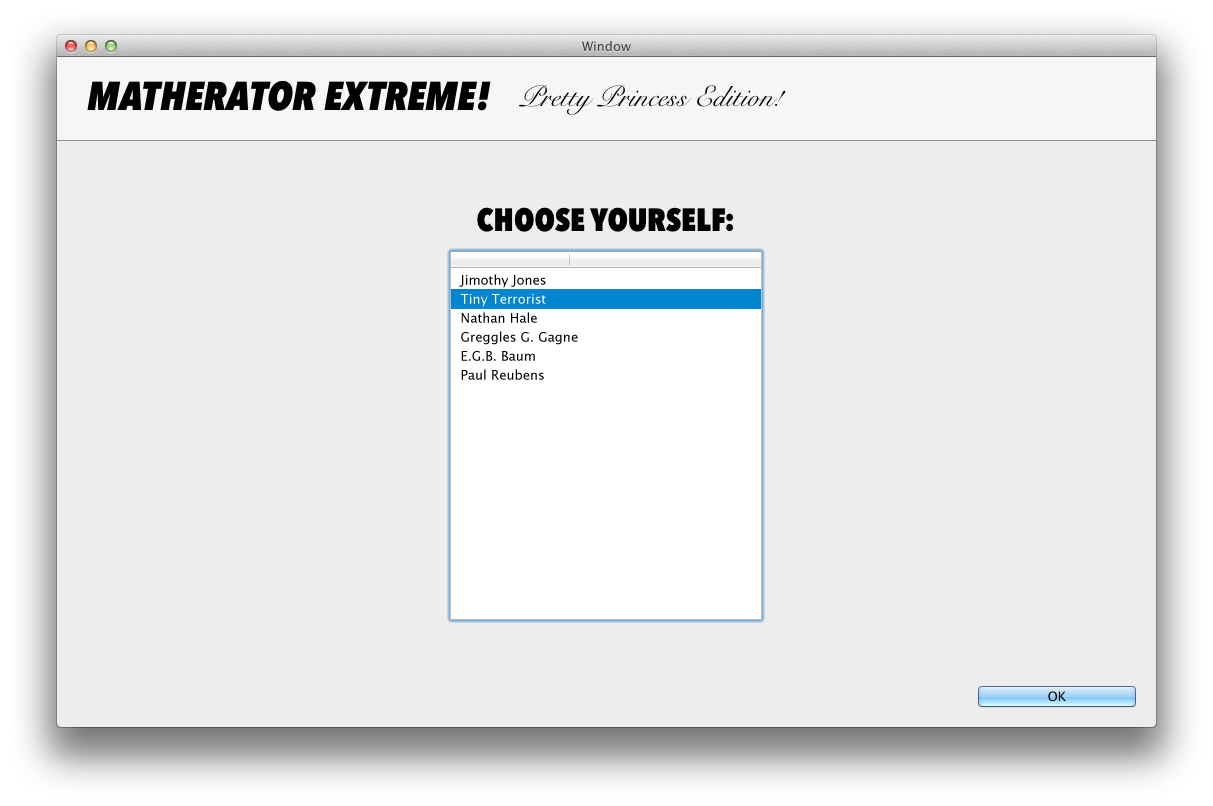
\includegraphics[width=13.59cm]{ChooseYourself}
    \captionof{figure}{The student log-in screen is shown only once; subsequently Matherator remembers the student.}
\end{center}

\begin{center}
    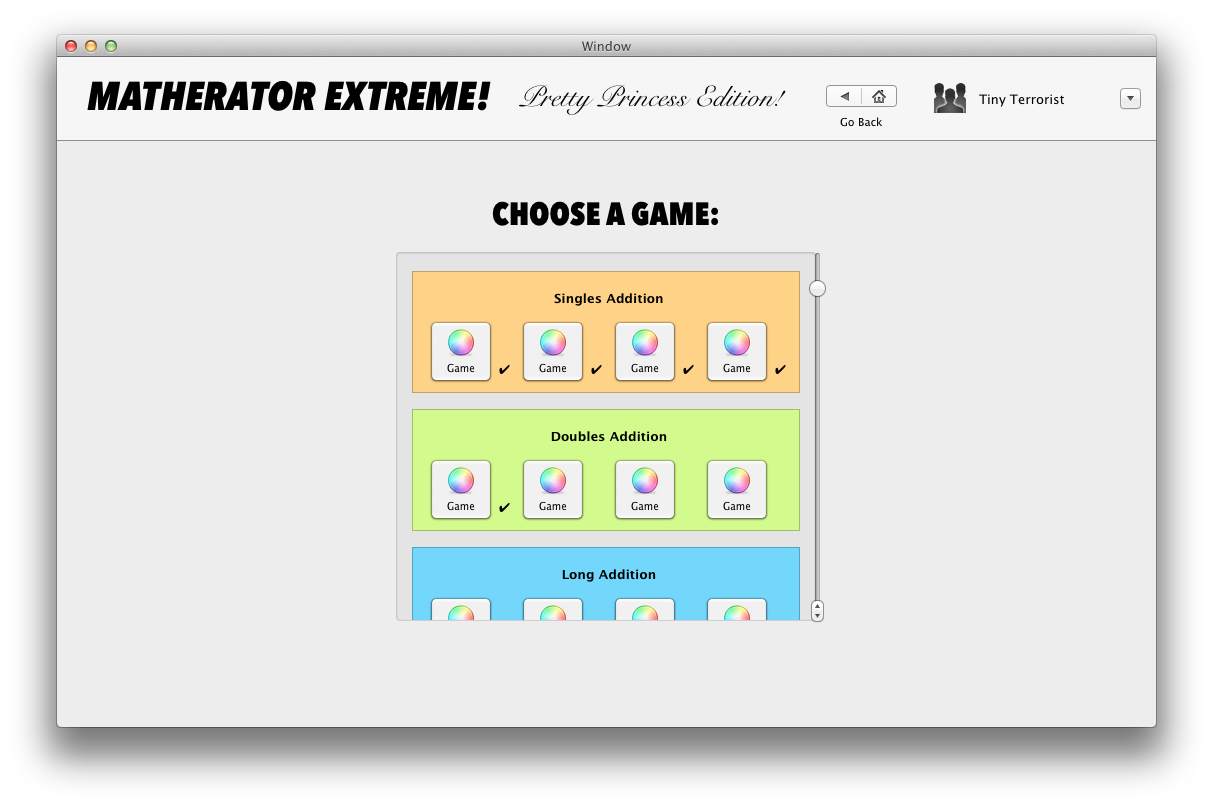
\includegraphics[width=13.59cm]{ChooseGame}
    \captionof{figure}{Student then chooses the game they want to play.}
\end{center}

\begin{center}
    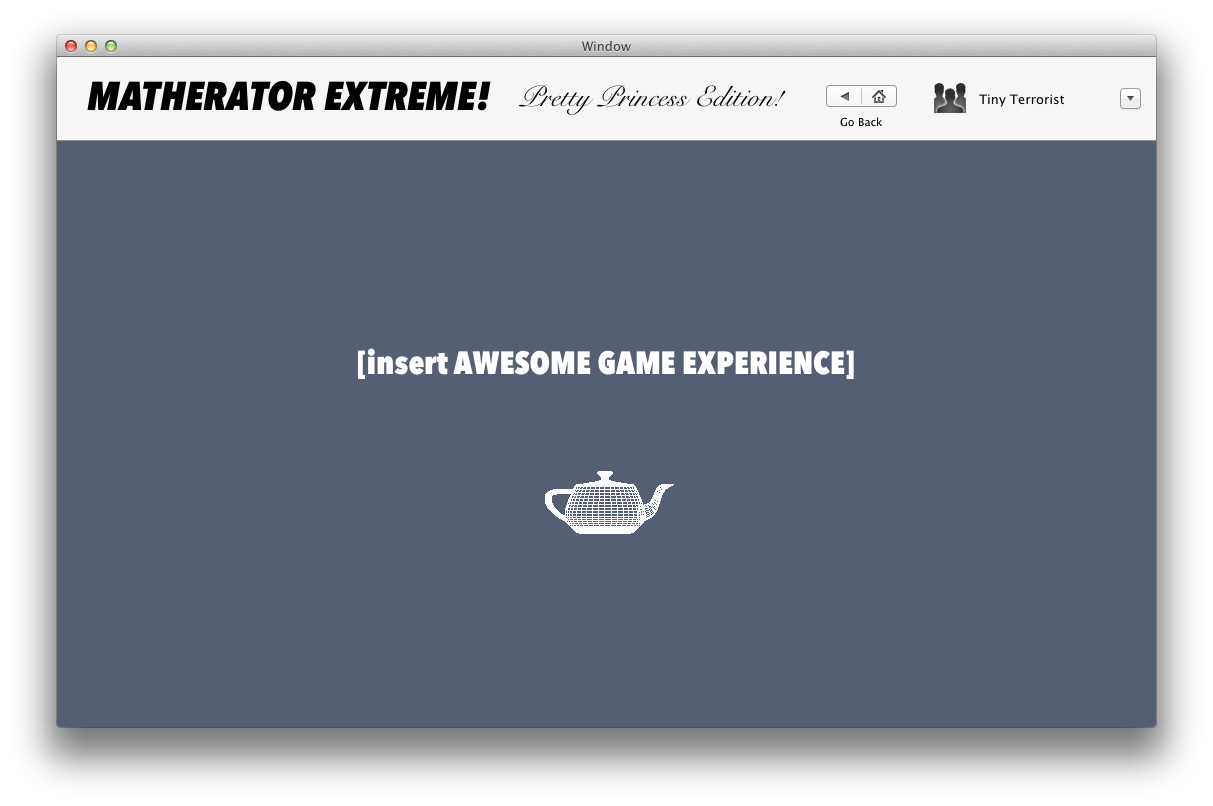
\includegraphics[width=13.59cm]{GameExperience}
    \captionof{figure}{Super-exciting placeholder gameplay.}
\end{center}








\chapter{Project Architecture}


\begin{figure}[hb]
    \centering
    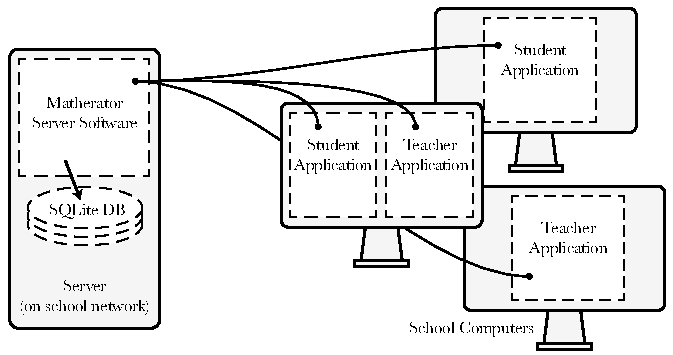
\includegraphics{OverarchingArchitecture}
    \caption{Overarching project architecture.}
    \label{fig:overarch}
\end{figure}


To maintain maximum interoperability between platforms, nearly all components of The Matherator will be written in Java.

The Student Component is a GUI-based desktop application built from a single-window philosophy. Standard Swing widgets will be used around the edges, but most of each game will be programmed using basic mouse- and key-listeners and basic drawing instructions.


\begin{figure}[htb]
    \centering
    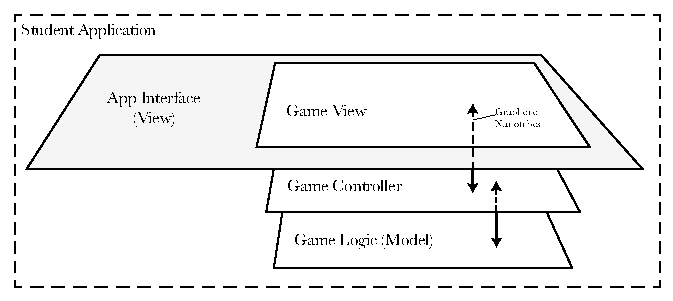
\includegraphics{MvcNoSrsly}
    \caption{It’s sensible MVC. No, seriously.}
    \label{fig:mvsee}
\end{figure}


For all the human interfaces we will be using a Model-View-Controller architecture, especially for the games:
\begin{itemize}
    \item The model will contain all of the logic for gameplay, and will be just modular enough so that parts of it can be reüsed between the different games.
    \item The views consist of the objects and sprites that draw themselves to the screen within the game.
    \item The controller (by definition) connects the views to the model, delivering digested and meaningful messages to the model in response to raw events from the views. It also receives update messages from the model and acts as a data supplier for view objects.
\end{itemize}
This is to facilitate sane implementation and maintenance, particularly in areas where rudimentary drawing instructions must be used.

The Teacher Component is also a GUI-based desktop application; in this case, only standard Swing widgets will be needed (still reasonably MVC-ish, of course).

The Server Component is a headless piece of software which maintains all its known teacher and student records in an SQLite database, which it controls directly.

The Student and Teacher software will communicate with the server in simple, record-based messages (encoded in YAML) over standard TCP connections—so it should go without saying that the computers running them need to be networked together.

At this point, on the client side, we are only providing for desktop-based applications. However, there is no reason that, in the future, these client components could not be adapted to mobile platforms.













\chapter{Project Requirements and Tasks}

Because of the length and relative dynamism of the \href{https://github.com/talusbb/matherator-extreme/wiki/User-Stories}{ \underline{project requirements document,}} it is housed on the Matherator project Wiki, in the form of a list of user stories.

Requirements will be added there as they are discovered, and shuffled between releases.

Similarly, \href{https://github.com/talusbb/matherator-extreme/wiki/Tasks}{ \underline{the list of tasks,}} as they relate to the development of the Matherator, are also maintained on the project Wiki, so that their status can be updated all the time.

















\end{document}
